\documentclass[border=4pt]{standalone}
\usepackage[T1]{fontenc}
\usepackage{tikz}
\usetikzlibrary{arrows.meta,positioning,fit,backgrounds,shapes.geometric,calc}
\definecolor{orch}{HTML}{234767}
\definecolor{ctx}{HTML}{EAF1F8}
\definecolor{retr}{HTML}{E2F0ED}
\definecolor{ext}{HTML}{F7EBDD}
\definecolor{infra}{HTML}{F1F3F5}
\tikzset{
 every node/.style={font=\sffamily\fontsize{8.5}{10}\selectfont,align=center},
 block/.style={draw=orch!80,fill=white,rounded corners=1.5pt,minimum height=7mm,inner sep=3pt,line width=.55pt},
 context/.style={block,fill=ctx},
 engine/.style={block,fill=orch,text=white},
 retrieval/.style={block,fill=retr},
 external/.style={block,fill=ext},
 storage/.style={block,fill=infra},
 flow/.style={-{Stealth[length=2mm]},draw=orch!90,line width=.65pt},
 control/.style={flow,dashed},
 error/.style={flow,densely dotted},
 group/.style={draw=orch!50,rounded corners=3pt,inner sep=5pt,line width=.5pt},
 heading/.style={font=\sffamily\bfseries\fontsize{8.5}{10}\selectfont,text=orch},
 edgelabel/.style={font=\sffamily\fontsize{7.5}{9}\selectfont,fill=white,inner sep=1pt,text=orch}
}

\begin{document}
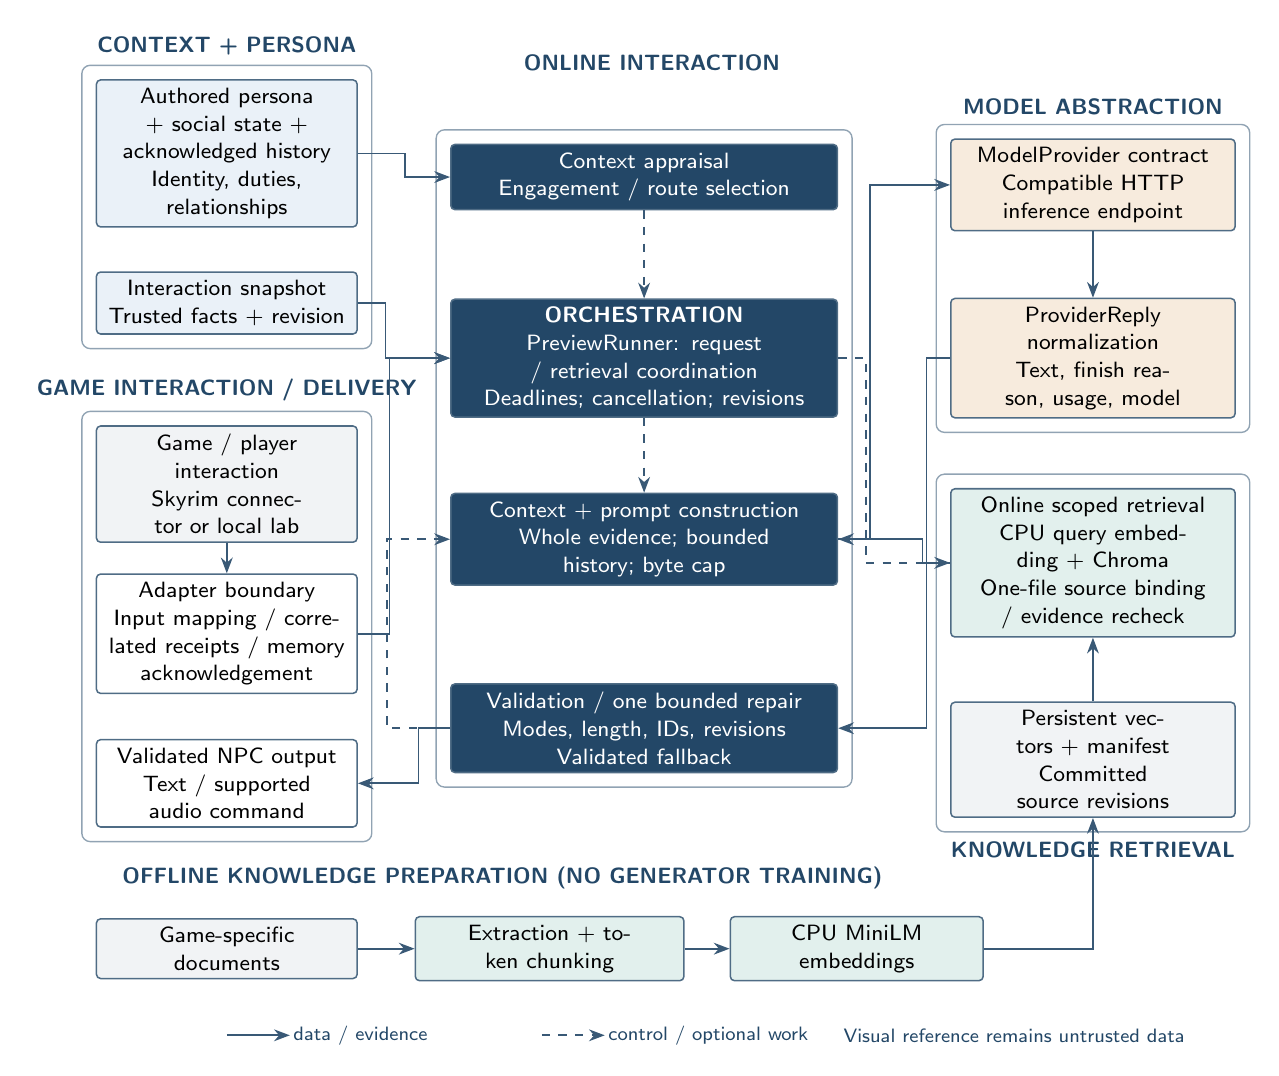
\begin{tikzpicture}
\node[context,text width=3.1cm] (persona) at (0,6.5) {Authored persona + social state + acknowledged history\\Identity, duties, relationships};
\node[context,text width=3.1cm] (snapshot) at (0,4.6) {Interaction snapshot\\Trusted facts + revision};
\node[storage,text width=3.1cm] (game) at (0,2.3) {Game / player interaction\\Skyrim connector or local lab};
\node[block,text width=3.1cm] (adapter) at (0,.4) {Adapter boundary\\Input mapping / correlated receipts / memory acknowledgement};
\node[block,text width=3.1cm] (output) at (0,-1.5) {Validated NPC output\\Text / supported audio command};
\node[engine,text width=4.7cm] (policy) at (5.3,6.2) {Context appraisal\\Engagement / route selection};
\node[engine,text width=4.7cm] (coord) at (5.3,3.9) {\textbf{ORCHESTRATION}\\PreviewRunner: request / retrieval coordination\\Deadlines; cancellation; revisions};
\node[engine,text width=4.7cm] (prompt) at (5.3,1.6) {Context + prompt construction\\Whole evidence; bounded history; byte cap};
\node[engine,text width=4.7cm] (validate) at (5.3,-.8) {Validation / one bounded repair\\Modes, length, IDs, revisions\\Validated fallback};
\node[external,text width=3.4cm] (provider) at (11,6.1) {ModelProvider contract\\Compatible HTTP inference endpoint};
\node[external,text width=3.4cm] (candidate) at (11,3.9) {ProviderReply normalization\\Text, finish reason, usage, model};
\node[retrieval,text width=3.4cm] (search) at (11,1.3) {Online scoped retrieval\\CPU query embedding + Chroma\\One-file source binding / evidence recheck};
\node[storage,text width=3.4cm] (index) at (11,-1.2) {Persistent vectors + manifest\\Committed source revisions};
\node[storage,text width=3.1cm] (docs) at (0,-3.6) {Game-specific documents};
\node[retrieval,text width=3.2cm] (parse) at (4.1,-3.6) {Extraction + token chunking};
\node[retrieval,text width=3.0cm] (embed) at (8,-3.6) {CPU MiniLM embeddings};
\node[heading] at (5.4,7.65) {ONLINE INTERACTION};
\node[heading] at (3.5,-2.7) {OFFLINE KNOWLEDGE PREPARATION (NO GENERATOR TRAINING)};
\draw[flow] (persona.east) -- ++(.6,0) |- (policy.west);
\draw[flow] (snapshot.east) -- ++(.35,0) |- (coord.west);
\draw[flow] (game) -- (adapter);
\draw[flow] (adapter.east) -- ++(.4,0) |- (coord.west);
\draw[control] (policy) -- (coord);
\draw[control] (coord) -- (prompt);
\draw[flow] (prompt.east) -- ++(.4,0) |- (provider.west);
\draw[flow] (provider) -- (candidate);
\draw[flow] (candidate.west) -- ++(-.3,0) |- (validate.east);
\draw[control] (coord.east) -- ++(.35,0) |- (search.west);
\draw[flow] (search.west) -- ++(-.35,0) |- (prompt.east);
\draw[flow] (index) -- (search);
\draw[flow] (validate.west) -- ++(-.4,0) |- (output.east);
\draw[control] (validate.west) -- ++(-.8,0) |- (prompt.west);
\draw[flow] (docs) -- (parse);
\draw[flow] (parse) -- (embed);
\draw[flow] (embed.east) -| (index.south);
\begin{pgfonlayer}{background}
\node[group,fit=(persona)(snapshot),label={[heading]above:CONTEXT + PERSONA}] {};
\node[group,fit=(game)(adapter)(output),label={[heading]above:GAME INTERACTION / DELIVERY}] {};
\node[group,fit=(policy)(coord)(prompt)(validate)] {};
\node[group,fit=(provider)(candidate),label={[heading]above:MODEL ABSTRACTION}] {};
\node[group,fit=(search)(index),label={[heading]below:KNOWLEDGE RETRIEVAL}] {};
\end{pgfonlayer}
\draw[flow] (0,-4.7) -- (.8,-4.7) node[edgelabel,right] {data / evidence};
\draw[control] (4,-4.7) -- (4.8,-4.7) node[edgelabel,right] {control / optional work};
\node[edgelabel] at (10,-4.7) {Visual reference remains untrusted data};
\end{tikzpicture}
\end{document}
